% !TEX program = lualatex
\documentclass[12pt,a4paper]{article}
\usepackage{amsmath,amssymb,amsthm}
\usepackage{geometry}
\geometry{margin=2.5cm}
\usepackage{hyperref}
\hypersetup{colorlinks=true,linkcolor=blue,citecolor=blue,urlcolor=blue}
\usepackage{booktabs}
\usepackage{lmodern}
\usepackage[T1]{fontenc}
\usepackage{graphicx}

\title{Realization of a Wave Packet Collapse Model\\in the Delay Circuit Model}
\author{Noriaki Kihara\\
WF System Co., Ltd.\\
Osaka University, School of Engineering Science (graduated)}
\date{April 2026\quad Research Note\\[4pt]
DOI: \href{https://doi.org/10.5281/zenodo.19534355}{10.5281/zenodo.19534355}}

\begin{document}

\maketitle

\begin{abstract}
This paper does not prove the physical mechanism of wave packet collapse. It extends the perfectly elastic collision framework defined in the previous paper \cite{ref4} and realizes behavior analogous to wave packet collapse on the delay circuit model. By treating the wave packet radius $r$ and the maximum wave height $w_{\max}$ as information, and by defining an operation function $*$ that causes $r$ to contract and $w_{\max}$ to increase upon collision, we construct a process in which a spread-out wave becomes localized through interaction.
\end{abstract}

\section{Introduction}

In the previous paper \cite{ref4}, perfectly elastic collisions were realized by class $F$. In this paper, we extend class $F$ from \cite{ref4} and define class $G$, in which the wave packet radius $r$ and the maximum wave height $w_{\max}$ are promoted to information.

What this paper demonstrates is the fact that, by adding to $*$ an operational rule under which $r$ contracts and $w_{\max}$ increases upon collision, behavior analogous to wave packet collapse can be constructed. This paper neither theoretically proves actual wave packet collapse nor contains any quantum-mechanical claims.

\section{Definition of Class $G$}

\subsection{Information and Meta-information}

In class $F$ of the previous paper \cite{ref4}, we promote $r$ (collision radius) and $w_{\max}$ (maximum wave height), which were meta-information, to information, and define class $G$.

\textbf{Information in class $G$:}
\begin{itemize}
  \item $i$: scalar value (input value)
  \item $w$: real value (amplitude)
  \item $x_0$: initial position
  \item $x$: current position
  \item $dx$: displacement
  \item $r$: wave packet radius (real number with $r > 0$)
  \item $w_{\max}$: maximum wave height (positive real number)
\end{itemize}

\textbf{Meta-information:}
\begin{itemize}
  \item $n$: counter (number of delays)
  \item $m$: wavelength (defined via $r$ by setting $m = r$)
  \item $F$: type (electron, photon, etc.)
  \item color: attribute for identification
\end{itemize}

\subsection{Mass Analogue}

The mass analogue is defined as $M = w_{\max} \cdot r$. $M$ is conserved before and after a collision.

\subsection{Operation Function $*$}

The updates to position and amplitude are identical to the previous paper \cite{ref4}:

\begin{equation}
  x = n \cdot dx + x_0
\end{equation}

\begin{equation}
  w = w_{\max} \cdot \sin\!\left(\frac{n}{m} \cdot 360°\right)
\end{equation}

\subsection{Collision Operations}

\subsubsection*{Interaction Rules}
\begin{itemize}
  \item Photon and photon: no interaction (pass through each other)
  \item Photon and electron: interact
\end{itemize}

\subsubsection*{Wave Packet Collapse}

When a collision occurs, the photon's $r$ is updated as follows:

\begin{equation}
  r^{\text{new}} = \min(r_1, r_2)
\end{equation}

Since $M = w_{\max} \cdot r$ is conserved, $w_{\max}$ increases as $r$ contracts:

\begin{equation}
  w_{\max}^{\text{new}} = \frac{M}{r^{\text{new}}} = \frac{w_{\max} \cdot r}{r^{\text{new}}}
\end{equation}

The wavelength is also updated: $m^{\text{new}} = r^{\text{new}}$.

\subsubsection*{Update of $dx$}

The update of $dx$ follows the perfectly elastic collision formula in \cite{ref4} \S5.1, using the mass analogue $M = w_{\max} \cdot r$:

\begin{equation}
  dx_1^{\text{new}} = \frac{(M_1 - M_2) \cdot dx_1 + 2\, M_2 \cdot dx_2}{M_1 + M_2}
\end{equation}

\begin{equation}
  dx_2^{\text{new}} = \frac{(M_2 - M_1) \cdot dx_2 + 2\, M_1 \cdot dx_1}{M_1 + M_2}
\end{equation}

\section{Sequence of Wave Packet Collapse}

\subsection{Definition of Instances}

Three instances are defined.

\textbf{$G_1$ (electron, red):}

\begin{table}[h]
\centering
\begin{tabular}{@{}ll@{}}
\toprule
Information / Meta-information & Value \\
\midrule
$x_0$ & 48 \\
$dx$ & 0 (at rest) \\
$r$ & 6 \\
$w_{\max}$ & 30 \\
$M = w_{\max} \cdot r$ & 180 \\
$F$ & electron \\
\bottomrule
\end{tabular}
\end{table}

\textbf{$G_2$ (photon, blue):}

\begin{table}[h]
\centering
\begin{tabular}{@{}ll@{}}
\toprule
Information / Meta-information & Value \\
\midrule
$x_0$ & 72 \\
$dx$ & $-8$ \\
$r$ & 48 \\
$w_{\max}$ & 1 \\
$M = w_{\max} \cdot r$ & 48 \\
$F$ & photon \\
\bottomrule
\end{tabular}
\end{table}

\textbf{$G_3$ (photon, green):}

\begin{table}[h]
\centering
\begin{tabular}{@{}ll@{}}
\toprule
Information / Meta-information & Value \\
\midrule
$x_0$ & 24 \\
$dx$ & $+8$ \\
$r$ & 48 \\
$w_{\max}$ & 1 \\
$M = w_{\max} \cdot r$ & 48 \\
$F$ & photon \\
\bottomrule
\end{tabular}
\end{table}

$G_2$ and $G_3$ are photons with a wide wave packet radius ($r = 48$), and $G_1$ is an electron with a narrow wave packet radius ($r = 6$). $G_1$ does not exist in the initial state; it is assumed to appear at $n = 3$ through external intervention (\cite{ref2} \S3.5).

\subsection{Before Collision ($n = 0, 1, 2$)}

$G_2$ and $G_3$ propagate independently. $G_1$ does not yet exist.

\begin{table}[h]
\centering
\begin{tabular}{@{}ccc@{}}
\toprule
$n$ & $x$ of $G_2$ & $x$ of $G_3$ \\
\midrule
0 & 72 & 24 \\
1 & 64 & 32 \\
2 & 56 & 40 \\
\bottomrule
\end{tabular}
\end{table}

Since $G_2$ and $G_3$ are both photons, they pass through each other without interacting.

\subsection{$n = 3$: External Intervention and Collision}

At $n = 3$, $G_1$ (electron) appears at $x = 48$ through external intervention.

The position of $G_2$ is $x = 48$, and the position of $G_3$ is $x = 48$, so all three reach the same position $x = 48$. A collision is determined from $(x_1 - x_2)^2 < \max(r_1^2, r_2^2)$.

\textbf{Wave packet collapse:}

\begin{equation}
  r^{\text{new}} = \min(48, 6) = 6
\end{equation}

\begin{equation}
  w_{\max}^{\text{new}} = \frac{48}{6} = 8
\end{equation}

\begin{equation}
  m^{\text{new}} = 6
\end{equation}

\textbf{Update of $dx$ (by symmetry):}

Since $G_2$ and $G_3$ collide with $G_1$ from symmetric positions and with symmetric velocities, the impulses on $G_1$ cancel each other, and $G_1$ remains at rest ($dx_1 = 0$).

\begin{equation}
  dx_2^{\text{new}} = \frac{(48 - 180)(-8) + 2 \cdot 180 \cdot 0}{48 + 180} = \frac{1056}{228} \approx +4.632
\end{equation}

\begin{equation}
  dx_3^{\text{new}} = \frac{(48 - 180)(+8) + 2 \cdot 180 \cdot 0}{48 + 180} = \frac{-1056}{228} \approx -4.632
\end{equation}

\subsection{After Collision ($n > 3$)}

\begin{table}[h]
\centering
\begin{tabular}{@{}cccc@{}}
\toprule
$n$ & $x$ of $G_1$ & $x$ of $G_2$ & $x$ of $G_3$ \\
\midrule
3  & 48.00 & 48.00 & 48.00 \\
4  & 48.00 & 52.63 & 43.37 \\
5  & 48.00 & 57.26 & 38.74 \\
6  & 48.00 & 61.89 & 34.11 \\
9  & 48.00 & 75.79 & 20.21 \\
12 & 48.00 & 89.68 &  6.32 \\
\bottomrule
\end{tabular}
\end{table}

$G_1$ (electron) remains at rest, while $G_2$ and $G_3$ (photons) move away in opposite directions as collapsed wave packets ($r = 6$, $w_{\max} = 8$, $m = 6$).

\subsection{Visualization of Wave Packet Collapse}

Below, the shape of the wave packets at each delay count $n$ is shown. The horizontal axis is position $x$ and the vertical axis is amplitude $w$.

$n = 0, 1, 2$: $G_2$ (blue) and $G_3$ (green) are spread throughout space as wide wave packets ($r = 48$, $w_{\max} = 1$).

$n = 3$: $G_1$ (electron, red) appears through external intervention and a collision occurs. The wave packets of $G_2$ and $G_3$ collapse to $r = 6$, $w_{\max} = 8$.

$n = 4, 5, \ldots, 12$: The collapsed $G_2$ and $G_3$ move away in opposite directions as narrow, tall wave packets.

\begin{figure}[h]
\centering
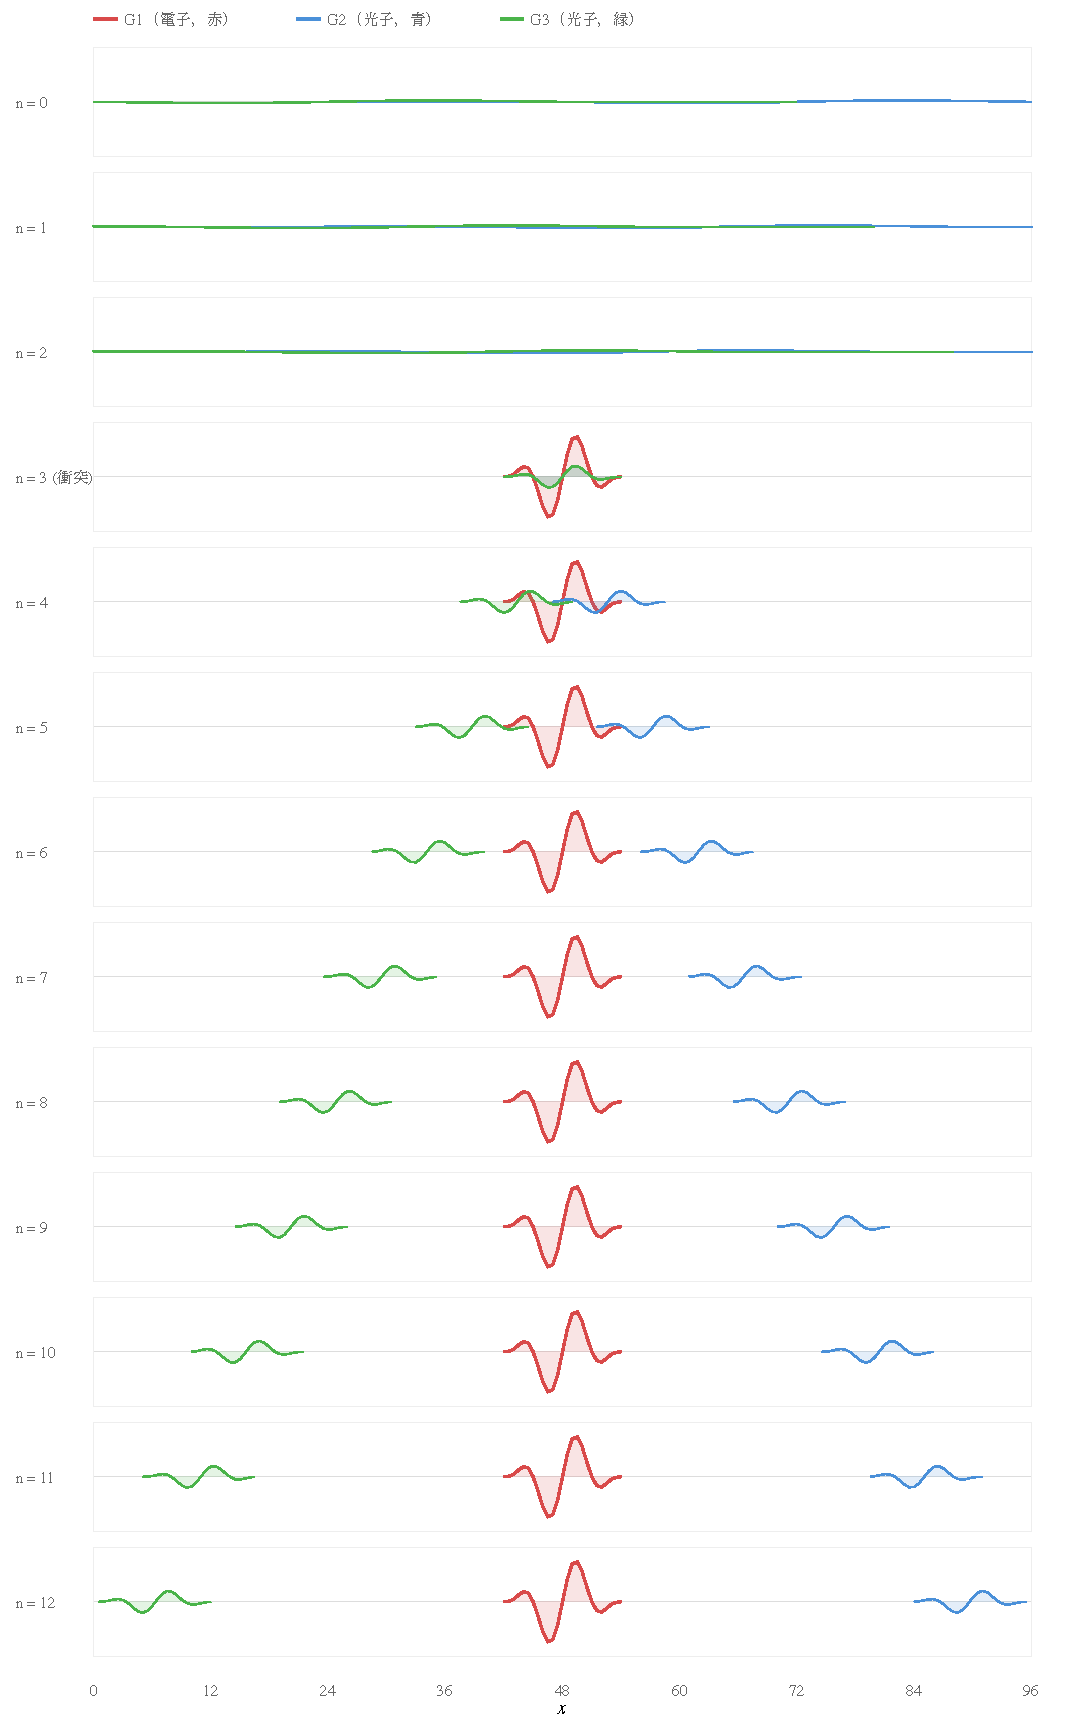
\includegraphics[width=0.85\textwidth]{fig11_wave_packet_collapse.pdf}
\caption{Wave Packet Collapse --- Shape change of wave packets from $n = 0$ to $n = 12$}
\label{fig:wave_packet_collapse}
\end{figure}

\section{Conclusion}

We extended class $F$ (perfectly elastic collisions) from the previous paper \cite{ref4} and defined class $G$, in which the wave packet radius $r$ and the maximum wave height $w_{\max}$ are promoted to information. Under conservation of the mass analogue $M = w_{\max} \cdot r$, we constructed an operational rule in which $r$ contracts and $w_{\max}$ increases upon collision.

We realized a process in which photons with wide wave packets ($r = 48$, $w_{\max} = 1$) collide with an electron having a narrow wave packet ($r = 6$), causing the wave packets to collapse ($r = 6$, $w_{\max} = 8$) and the wavelength to shorten ($m = 6$). This is behavior analogous to wave packet collapse, but it contains no quantum-mechanical claims.

\begin{thebibliography}{9}

\bibitem{ref1}
Noriaki Kihara,
``Information-Theoretic Organization of Information Transmission,''
Research Note, April 2026.

\bibitem{ref2}
Noriaki Kihara,
``Organization of Symmetries Inherent in the Delay Circuit Model,''
Research Note, April 2026.

\bibitem{ref3}
Noriaki Kihara,
``Realization of Simple Harmonic Oscillation and Sinusoidal Waves in the Delay Circuit Model,''
Research Note, April 2026.

\bibitem{ref4}
Noriaki Kihara,
``Realization of Perfectly Elastic Collisions in the Delay Circuit Model,''
Research Note, April 2026.

\end{thebibliography}

\end{document}
